\chapter{Advanced Spring Data JPA}


TODO relationships again

\section{Relationships}

JPA supports the same associations as you know from relational databases.

 You can use:
\begin{itemize}
\item one-to-one associations,
\item many-to-one associations and
\item many-to-many associations.
\end{itemize}
You can map each of them as a uni- or bidirectional association.


\subsection{One-to-One relationship}

In a one-to-one relationship, one record in a table is associated with one and only one record in another table.

\begin{lstlisting}[frame=single, language=java]
package be.pxl.paj.domain;

import javax.persistence.Entity;
import javax.persistence.GeneratedValue;
import javax.persistence.GenerationType;
import javax.persistence.Id;
import javax.persistence.Table;

@Entity
@Table(name = "contact_info")
public class ContactInformation {
	@Id
	@GeneratedValue(strategy = GenerationType.IDENTITY)
	private Long id;
	private String phone;
	private String email;
	private String linkedIn;

	public ContactInformation() {
	}

	public Long getId() {
		return id;
	}

	public String getPhone() {
		return phone;
	}

	public void setPhone(String phone) {
		this.phone = phone;
	}

	public String getEmail() {
		return email;
	}

	public void setEmail(String email) {
		this.email = email;
	}

	public String getLinkedIn() {
		return linkedIn;
	}

	public void setLinkedIn(String linkedIn) {
		this.linkedIn = linkedIn;
	}
}
\end{lstlisting}

The member variable with the type of the associated entity class is annotated with @OneToOne. You can customize the name of the foreign key column with a @JoinColumn annotation.

\begin{lstlisting}[frame=single, language=java]
package be.pxl.paj.domain;

import javax.persistence.CascadeType;
import javax.persistence.Column;
import javax.persistence.Entity;
import javax.persistence.GeneratedValue;
import javax.persistence.GenerationType;
import javax.persistence.Id;
import javax.persistence.OneToOne;

@Entity
public class Researcher {

	@Id
	@GeneratedValue(strategy = GenerationType.IDENTITY)
	private Long id;
	@Column(length = 40, nullable = false)
	private String name;
	@OneToOne(cascade = CascadeType.ALL)
	private ContactInformation contactInformation;

	public Long getId() {
		return id;
	}

	public String getName() {
		return name;
	}

	public void setName(String name) {
		this.name = name;
	}

	public ContactInformation getContactInformation() {
		return contactInformation;
	}

	public void setContactInformation(ContactInformation contactInformation) {
		this.contactInformation = contactInformation;
	}
}
\end{lstlisting}

The meaning of CascadeType.ALL is that the persistence context will propagate (cascade) all EntityManager operations (PERSIST, REMOVE, REFRESH, MERGE, DETACH) to the relating entities.

\subsection{Many-to-one relationship}

Next an example of a many-to-one relationship.  
Suppose there are multiple researchers working on one project, but every researcher is assigned to one project. 

Here is the entity class Project.

\begin{lstlisting}[frame=single, language=java]
package be.pxl.paj.domain;

import javax.persistence.Entity;
import javax.persistence.GeneratedValue;
import javax.persistence.GenerationType;
import javax.persistence.Id;
import java.time.LocalDate;

@Entity
public class Project {
	@Id
	@GeneratedValue(strategy = GenerationType.IDENTITY)
	private Long id;
	private String name;
	private LocalDate start;
	@Enumerated(value= EnumType.STRING)
	private ProjectPhase projectPhase;

	public Project() {
	}

	public Project(String name, LocalDate start) {
		this.name = name;
		this.start = start;
	}

	public Long getId() {
		return id;
	}

	public void setId(Long id) {
		this.id = id;
	}

	public String getName() {
		return name;
	}

	public void setName(String name) {
		this.name = name;
	}

	public LocalDate getStart() {
		return start;
	}

	public void setStart(LocalDate start) {
		this.start = start;
	}
	
	public ProjectPhase getProjectPhase() {
		return projectPhase;
	}

	public void setProjectPhase(ProjectPhase projectPhase) {
		this.projectPhase = projectPhase;
	}
}
\end{lstlisting}

\begin{lstlisting}[frame=single, language=java]
package be.pxl.paj.domain;

public enum ProjectPhase {
	INITIATING,
	PLANNING,
	EXECUTING,
	CLOSING;
}
\end{lstlisting}

The most common option to map an enum value to and from its database representation in JPA is to use the @Enumerated annotation. This way, we can instruct a JPA provider to convert an enum to its ordinal or String value.  When using the String value,  we can safely add new enum values or change our enum's order.  However, renaming an enum value will still break the database data.

To create the relation between a researcher and the project he's working on, we add a @ManyToOne relationship in the entity class Researcher.

\begin{lstlisting}[frame=single,language=java]
package be.pxl.paj.domain;

import javax.persistence.CascadeType;
import javax.persistence.Column;
import javax.persistence.Entity;
import javax.persistence.GeneratedValue;
import javax.persistence.GenerationType;
import javax.persistence.Id;
import javax.persistence.ManyToOne;
import javax.persistence.OneToOne;

@Entity
public class Researcher {

	@Id
	@GeneratedValue(strategy = GenerationType.IDENTITY)
	private Long id;
	@Column(length = 40, nullable = false)
	private String name;
	@OneToOne(cascade = CascadeType.ALL)
	private ContactInformation contactInformation;
	@ManyToOne
	private Project project;

	public Long getId() {
		return id;
	}

	public String getName() {
		return name;
	}

	public void setName(String name) {
		this.name = name;
	}

	public ContactInformation getContactInformation() {
		return contactInformation;
	}

	public void setContactInformation(ContactInformation contactInformation) {
		this.contactInformation = contactInformation;
	}

	public void setProject(Project project) {
		this.project = project;
	}

	public Project getProject() {
		return project;
	}
}
\end{lstlisting}

At the moment, it's not possible to see which researchers are working on a project. To make this possible we have to make the relationship between project and researcher bi-directional.  Researcher is defined the \textbf{owner} of the relationship. To make this association bi-directional, all we'll have to do is to define the referencing side. The inverse or the referencing side simply maps to the owning side.  The value of mappedBy is the name of the association-mapping attribute on the owning side.  The fetch type of this @OneToMany relationship is by default \textbf{lazy}. This means the researcher for a project are only retrieved from the database when the getResearchers() method is called.

\begin{lstlisting}[frame=single, language=java]
package be.pxl.paj.domain;

import javax.persistence.Entity;
import javax.persistence.GeneratedValue;
import javax.persistence.GenerationType;
import javax.persistence.Id;
import javax.persistence.OneToMany;
import java.time.LocalDate;
import java.util.ArrayList;
import java.util.List;

@Entity
public class Project {
	@Id
	@GeneratedValue(strategy = GenerationType.IDENTITY)
	private Long id;
	private String name;
	private LocalDate start;
	@OneToMany(mappedBy = "project")
	private List<Researcher> researchers = new ArrayList<>();

	public Project() {
	}

	public Project(String name) {
		this.name = name;
		this.start = LocalDate.now();
	}

	public Long getId() {
		return id;
	}

	public void setId(Long id) {
		this.id = id;
	}

	public String getName() {
		return name;
	}

	public void setName(String name) {
		this.name = name;
	}

	public LocalDate getStart() {
		return start;
	}

	public void setStart(LocalDate start) {
		this.start = start;
	}

	public List<Researcher> getResearchers() {
		return researchers;
	}

	public void addResearcher(Researcher researcher) {
		researchers.add(researcher);
	}

	public void removeResearcher(Researcher researcher) {
		researchers.remove(researcher);
	}

	@Override
	public String toString() {
		return name;
	}
}
\end{lstlisting}


\begin{oefening}
Use the programs CreateResearcherApp, CreateProjectApp and AssignResearcherApp to create some sample data.
Use the program ProjectDetailsApp to retrieve the details of a project.  Now, change the fetch type of the @OneToMany relationship to eager and retrieve the project details again. What can you tell about the queries being executed?
\end{oefening}
 
It's not a good idea to make Project owner of the relationship between Projects and Researchers.  You may end up with an inefficient database schema. More information can be found in this post: \url{https://vladmihalcea.com/the-best-way-to-map-a-onetomany-association-with-jpa-and-hibernate/}.


\subsection{Many-to-many relationship}

Actually, we want our researchers to work on multiple projects. Therefore,  we have to introduce a @ManyToMany relationship in the class Researcher. 

\begin{lstlisting}[frame=single,language=java]
package be.pxl.paj.domain;

import org.apache.logging.log4j.LogManager;
import org.apache.logging.log4j.Logger;

import javax.persistence.CascadeType;
import javax.persistence.Column;
import javax.persistence.Entity;
import javax.persistence.GeneratedValue;
import javax.persistence.GenerationType;
import javax.persistence.Id;
import javax.persistence.ManyToMany;
import javax.persistence.OneToOne;
import java.util.ArrayList;
import java.util.List;

@Entity
public class Researcher {

	private static final Logger LOGGER = LogManager.getLogger(Researcher.class);

	@Id
	@GeneratedValue(strategy = GenerationType.IDENTITY)
	private Long id;
	@Column(length = 40, nullable = false)
	private String name;
	@OneToOne(cascade = CascadeType.ALL)
	private ContactInformation contactInformation;
	@ManyToMany
	private List<Project> projects = new ArrayList<>();

	public Long getId() {
		return id;
	}

	public String getName() {
		return name;
	}

	public void setName(String name) {
		this.name = name;
	}

	public ContactInformation getContactInformation() {
		return contactInformation;
	}

	public void setContactInformation(ContactInformation contactInformation) {
		this.contactInformation = contactInformation;
	}

	public void addProject(Project project) {
		if (this.projects.contains(project)) {
				LOGGER.info("Researcher [" + name + "] already assigned to [" + project.getName() + "]");
				return;
		}
		this.projects.add(project);
		project.addResearcher(this);
	}

	public List<Project> getProjects() {
		return projects;
	}

	@Override
	public String toString() {
		return "Researcher{" +
				"id=" + id +
				", name='" + name + '\'' +
				", contactInformation=" + contactInformation +
				'}';
	}
}
\end{lstlisting}



If we want the relationship to be bi-directional, Researcher remains the owner of the relationship.  

\begin{lstlisting}[frame=single,language=java]
package be.pxl.paj.domain;

import javax.persistence.Entity;
import javax.persistence.GeneratedValue;
import javax.persistence.GenerationType;
import javax.persistence.Id;
import javax.persistence.ManyToMany;
import java.time.LocalDate;
import java.util.ArrayList;
import java.util.List;

@Entity
public class Project {
	@Id
	@GeneratedValue(strategy = GenerationType.IDENTITY)
	private Long id;
	private String name;
	private LocalDate start;
	@ManyToMany(mappedBy = "projects")
	private List<Researcher> researchers = new ArrayList<>();

	public Project() {
	}

	public Project(String name) {
		this.name = name;
		this.start = LocalDate.now();
	}

	public Long getId() {
		return id;
	}

	public void setId(Long id) {
		this.id = id;
	}

	public String getName() {
		return name;
	}

	public void setName(String name) {
		this.name = name;
	}

	public LocalDate getStart() {
		return start;
	}

	public void setStart(LocalDate start) {
		this.start = start;
	}

	public List<Researcher> getResearchers() {
		return researchers;
	}

	@Override
	public boolean equals(Object o) {
		if (this == o) {
			return true;
		}
		if (o == null || getClass() != o.getClass()) {
			return false;
		}

		Project project = (Project) o;

		return id != null ? id.equals(project.id) : project.id == null;
	}

	@Override
	public int hashCode() {
		return id != null ? id.hashCode() : 0;
	}

	public void addResearcher(Researcher researcher) {
		researchers.add(researcher);
	}

	@Override
	public String toString() {
		return name;
	}
}
\end{lstlisting}


When you execute one of the programs and look at the created database schema, you will notice that a \textbf{link table} is created for storing the many-to-many relationship.

\begin{oefening}
Implement the bi-directional many-to-many relationship between Researchers and Projects in the SampleJPAProject. Create a new program to remove a researcher from a project.  Make sure all data is managed correctly by the owner of the relationship.
\end{oefening}


\section{N + 1 query problem}

We have the entity-class Post and the entity-class PostComment. There is a uni-directional many-to-one relationship between PostComment and Post.  A PostComment belongs to exactly one Post however for one Post there may exist multiple PostComments.

\begin{lstlisting}[frame=single,  language=java]
package be.pxl.paj.domain.posts;

import javax.persistence.Entity;
import javax.persistence.GeneratedValue;
import javax.persistence.Id;

@Entity
public class Post {
	@Id
	@GeneratedValue
	private Long id;
	private String title;

	public Post() {
		// JPA only
	}

	public Post(String title) {
		this.title = title;
	}

	public Long getId() {
		return id;
	}

	public String getTitle() {
		return title;
	}

	public void setTitle(String title) {
		this.title = title;
	}
}
\end{lstlisting}

\begin{lstlisting}[frame=single,  language=java]
package be.pxl.paj.domain.posts;

import javax.persistence.Entity;
import javax.persistence.GeneratedValue;
import javax.persistence.Id;
import javax.persistence.ManyToOne;

@Entity
public class PostComment {
	@Id
	@GeneratedValue
	private Long id;
	@ManyToOne
	private Post post;
	private String review;

	public PostComment() {
		// JPA only
	}
	public PostComment(Post post, String review) {
		this.post = post;
		this.review = review;
	}

	public Long getId() {
		return id;
	}

	public Post getPost() {
		return post;
	}

	public void setPost(Post post) {
		this.post = post;
	}

	public String getReview() {
		return review;
	}

	public void setReview(String review) {
		this.review = review;
	}
}
\end{lstlisting}

Here's a naive implementation of a program that retrieves all the comments from the database.  For every retrieved comment, the title of the original post is displayed as well.

\begin{lstlisting}[frame=single,  language=java]
package be.pxl.paj;

import be.pxl.paj.domain.posts.Post;
import be.pxl.paj.domain.posts.PostComment;

import javax.persistence.EntityManager;
import javax.persistence.EntityManagerFactory;
import javax.persistence.Persistence;
import javax.persistence.Query;
import java.util.List;

public class PostWithComments {

	public static void main(String[] args) throws Exception {

		EntityManagerFactory emf = Persistence.createEntityManagerFactory("musicdb_pu");
		EntityManager em = emf.createEntityManager();

		List<PostComment> comments = em.createQuery("select pc from PostComment pc", PostComment.class).getResultList();
		
		for (PostComment comment : comments) {
			System.out.println(comment.getReview() + " on " + comment.getPost().getTitle());
		}

		em.close();
		emf.close();
	}

}
\end{lstlisting}

You may expect that only one query is sufficient for retrieving this data. However, if you look at the actual queries being executed, you find out there are multiple queries needed. That's not efficient! This problem is known as the N+1-problem.  There is one query for retrieving the comments and N queries for retrieving the accompanying post.

The solution is rewriting the query to retrieve the comments and posts at once. 

\begin{lstlisting}[frame=single,  language=java]
package be.pxl.paj;

import be.pxl.paj.domain.posts.Post;
import be.pxl.paj.domain.posts.PostComment;

import javax.persistence.EntityManager;
import javax.persistence.EntityManagerFactory;
import javax.persistence.Persistence;
import javax.persistence.Query;
import java.util.List;

public class PostWithComments {

	public static void main(String[] args) throws Exception {

		EntityManagerFactory emf = Persistence.createEntityManagerFactory("musicdb_pu");
		EntityManager em = emf.createEntityManager();

		List<PostComment> comments = em.createQuery("select pc from PostComment pc join fetch pc.post p", PostComment.class).getResultList();
		
		for (PostComment comment : comments) {
			System.out.println(comment.getReview() + " on " + comment.getPost().getTitle());
		}

		em.close();
		emf.close();
	}

}
\end{lstlisting}


\section{Exercises}

\begin{oefening}
Implement the entity classes Artist, Album and Song. The relationships between these classes (and the corresponding tables) are shown in the figure below.  Implement these relationships in a bi-directional way.

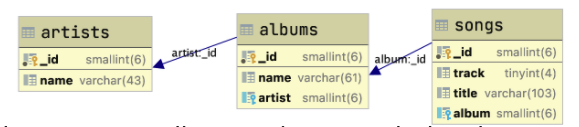
\includegraphics[width=\textwidth]{./images/chapter6/exercise-schema}

Implement the interface ArtistDao and it's implementation ArtistDaoImpl. The methods you need to implement can be found in the class diagram.

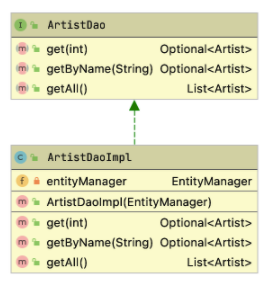
\includegraphics{./images/chapter6/exercise-dao}

Write unit tests for the class ArtistDaoImpl.

Create the program ArtistApp. A user can input the name of an artist. The program displays all the albums of the artist. For each album the songs are displayed ordered by track number.
\end{oefening}


\begin{oefening}
\textbf{Optional:} 
https://github.com/bobocode-projects/jpa-hibernate-exercises/tree/master/photo-comment-dao
\end{oefening}